\section{Conventional Three Level Boost Converter}\label{ch:TLBC}

The conventional three level boost converter is the first variation of the conventional BC that includes not only passive components, but also an additional active component. This, opposite to all other topologies discussed,does not increase the ratio between output and input, as it will be proven in the this section, but provides lower stress, low inductor current ripple and low switching loss compared to the conventional BC. 

\subsection{Additions from Conventional BC}
In the CTLBC, a second switch is included, together with another capacitor to go in parallel with it, An additional diode is included to allow both switches to conduct at the same time without causing damage to the circuit. The full schematic can be seen on Fig. \ref{fig:CTLBC}  

\begin{figure} [H]
   \centering
   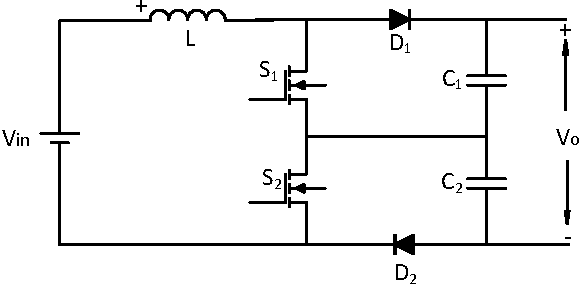
\includegraphics[width=0.6\textwidth]{figures/dConventionalThreeLevelBC/Three_level.pdf}
    \caption{Conventional Three Level Boost Converter circuit}
	\label{fig:CTLBC}
\end{figure}
\subsection{Switching States}
<<<<<<< Updated upstream
As there are two switches in this topology, a different switching pattern is required in comparison to the Conventional BC. The pattern of choice is shifting the signal of the second switch by an of angle 90$^\circ$ degrees.
=======
As there are two switches in this topology, a different switching pattern is required in comparison to the Conventional BC. The pattern of choice is shifting the signal to the second switch by 90$^\circ$ degrees.
>>>>>>> Stashed changes
In this case, there are four possible states, corresponding to all possible combinations between the switches. Not all of them occur for one given duty cycle value. 
The equivalent circuits during the on and off stages are shown in Figure \ref{fig:CTLBC_States}. Here again we assume the capacitors are the same size and that the duty ratio applied to the two switches is the same. 
\vspace{-5mm}
\begin{figure}[H]%
    \centering
    \subfloat[Switch S\textsubscript{1} ON, Switch S\textsubscript{2} ON\label{CTLBC_ONON}]
    {{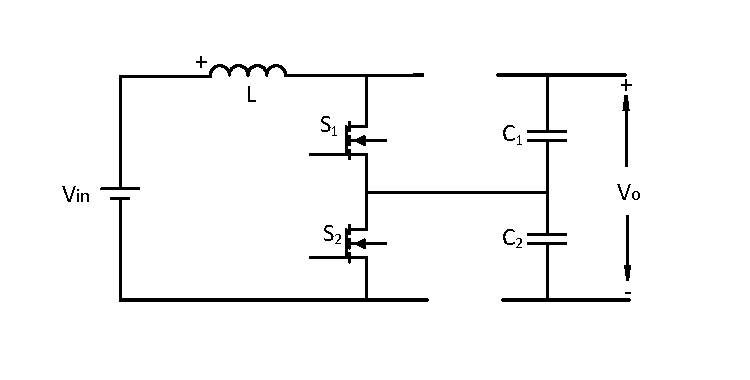
\includegraphics[width=0.45\textwidth]{figures/dConventionalThreeLevelBC/Three_levelONON.pdf} }}%
    \qquad
    \subfloat[Switch S\textsubscript{1} ON, Switch S\textsubscript{2} OFF\label{CTLBC_ONOFF}]{{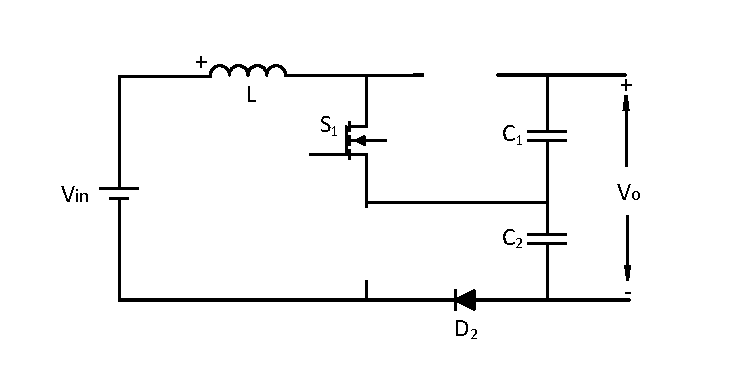
\includegraphics[width=0.45\textwidth]{figures/dConventionalThreeLevelBC/Three_levelONOFF.pdf} }}%  
   \qquad
        \subfloat[Switch S\textsubscript{1} OFF, Switch S\textsubscript{2} ON\label{CTLBC_OFFON}]
    {{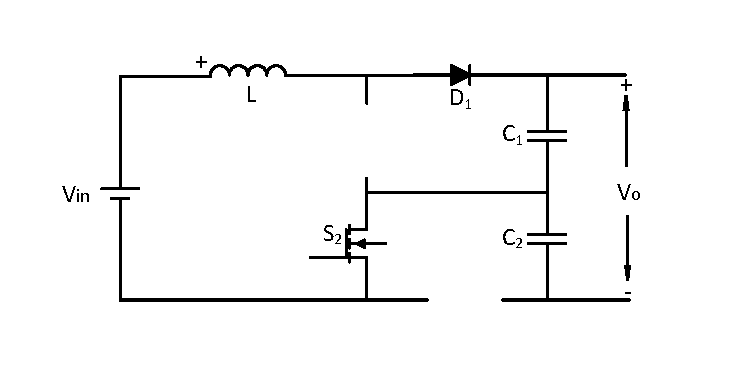
\includegraphics[width=0.45\textwidth]{figures/dConventionalThreeLevelBC/Three_levelOFFON.pdf} }}%
    \qquad
    \subfloat[Switch S\textsubscript{1} OFF, Switch S\textsubscript{2} OFF\label{CTLBC_OFFOFF}]{{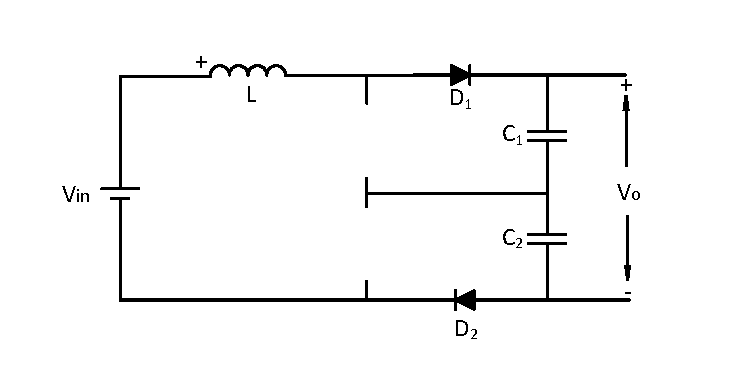
\includegraphics[width=0.45\textwidth]{figures/dConventionalThreeLevelBC/Three_levelOFFOFF.pdf} }}%  
    \caption{Switching states of the SIBC}%
     \label{fig:CTLBC_States}% 
     
\end{figure}
\subsubsection{Switch S\textsubscript{1} ON, Switch S\textsubscript{2} ON State}
Here we have got a replica of the ON state of a conventional boost converter, as both switches conduct and both diodes are reverse biased. (Can be seen on Figure \ref{CTLBC_ONON}) A loop is formed with the inductor and the power supply. We use KVL to express the voltage over the inductor as: 

\begin{equation}
	V_{L}=V_{in}
	\label{eq:CTLBC_KVL_ONON}
\end{equation}
<<<<<<< Updated upstream
Another loop is formed with the two capacitor and the output. This loop can be observed over all the rest of the states as well. Again assuming the capacitors are the same size, the voltage would split equally across them and the loop can be expressed via KVL as: 
=======
Another loop is formed with the two capacitors and the output.This loop can be observed over all the rest of the states as well and can be expressed via KVL as: 
>>>>>>> Stashed changes

\begin{equation}
	V_O=V_{C_1}+V_{C_2}
	\label{eq:CTLBC_KVL_ONON2}
\end{equation}


\subsubsection{Switch S\textsubscript{1} ON, Switch S\textsubscript{2} OFF State}
While only switch S\textsubscript{1} conducts, diode D\textsubscript{2} is forwards biased and extends the loop over C\textsubscript{2}. (Can be seen on Figure \ref{CTLBC_ONOFF}) We use KVL to express the voltage over the inductor as: 
\begin{equation}
	V_{L}=V_{in}-V_{C_1}
	\label{eq:CTLBC_KVL_ONOFF}
\end{equation}
 
\subsubsection{Switch S\textsubscript{1} OFF, Switch S\textsubscript{2} ON State}
Similar to the previous state, S\textsubscript{2} conducts, diode D\textsubscript{1} is forwards biased and extends the loop over C\textsubscript{1} (Can be seen on Figure \ref{CTLBC_OFFON}). As already stated, capacitor sizes and duty cycles are assumed equal, therefore no change in KVL between the two loops: 
\begin{equation}
	V_{L}=V_{in}-V_{C_2}
	\label{eq:CTLBC_KVL_OFFON}
\end{equation}

\subsubsection{Switch S\textsubscript{1} OFF, Switch S\textsubscript{2} OFF State}
With both switches open the circuit formed is equivalent to the OFF state in a conventional BC. (Can be seen on Figure \ref{CTLBC_OFFOFF}) We use KVL to express the voltage over the inductor as: 
\begin{equation}
	V_{L}=V_{in}-V_{O}
	\label{eq:CTLBC_KVL_OFFOFF}
\end{equation}

<<<<<<< Updated upstream
To find an expression for the output-input gain of the topology, we refer back to the IVSB (Sec. \ref{sec:convertionRatio}) and formulate the expression that is valid for both switches since Eq. \ref{eq:CTLBC_KVL_ONOFF} and Eq. \ref{eq:CTLBC_KVL_OFFON} are identical:
=======
To find an expression for the output-input gain of the topology, we 
have to observe two separate cases. First, when the duty cycle is above 0.5, state (d) never occurs as at any time one of the switches is on. We have an equal split of states (b) and (c) for a duration of $(1-D)T_S$, whit state (a) lasting for the rest of the cycle or $1-(1-D)=2(D-1)$.

The second case is when $D<0.5$. In that case state (a) never occurs, while states (b) and (c) last for the duty cycle duration $D$. State (d) lasts for the rest of the cycle or $(1-2D)$.
Now we can refer back to the IVSB and build two separate equations for the two cases. 

Case 1: 
>>>>>>> Stashed changes
\begin{equation}
	V_{L_a}(2D-1)+V_{L_b}(1-D)+V_{L_b}(1-D)=
	\label{eq:CTLBC_IVSB}
\end{equation}
Substituting the already derived expressions for V\textsubscript{L}:

\begin{equation}
	V_{in}(2D-1)+(V_{in} - V_{C_1})(1-D)+(V_{in} - V_{C_2})(1-D)=0
	\label{eq:CTLBC_IVSB2}
\end{equation}
Reforming this equation we get: 

\begin{equation}
	V_{in}=(V_{C_1} - V_{C_2})(1-D)
	\label{eq:CTLBC_IVSB3}
\end{equation}
<<<<<<< Updated upstream
Using the already derived expression for V\textsubscript{O} in Eq. \ref{eq:CTLBC_KVL_ONON2} we can directly form the output-input function: 
=======
Now we substitute from Eq.\ref{eq:CTLBC_KVL_ONON2}:

>>>>>>> Stashed changes
\begin{equation}
	V_{in}=(V_{O})(1-D)
	\label{eq:CTLBC_IVSB4}
\end{equation}
From here the output-input function is easily found:

\begin{equation}
	\frac{V_O}{V_{in}}=\frac{1}{(1-D)}
	\label{eq:CTLBC_IVSB5}
\end{equation}

Case 2: 
\begin{equation}
	V_{L_d}(1-2D)+V_{L_b}D+V_{L_b}D=
	\label{eq:CTLBC_CASE2}
\end{equation}
Substituting the already derived expressions for V\textsubscript{L}:

\begin{equation}
	(V_{in}-V_O)(1-2D)+(V_{in} - V_{C_1})D+(V_{in} - V_{C_2})D=0
	\label{eq:CTLBC_CASE2_2}
\end{equation}
Reforming this equation we get: 

\begin{equation}
	V_{in}=(V_{C_1} - V_{C_2})D+V_O(1-2D)
	\label{eq:CTLBC_CASE2_3}
\end{equation}
Again, we substitute from Eq.\ref{eq:CTLBC_KVL_ONON2}:

\begin{equation}
	V_{in}=V_{O}(1-D)
	\label{eq:CTLBC_CASE2_4}
\end{equation}
And the relationship is derived to be the same as in Case 1:

\begin{equation}
	\frac{V_O}{V_{in}}=\frac{1}{(1-D)}
	\label{eq:CTLBC_CASE2_5}
\end{equation}

Now it can be confirmed, the gain of the CTLBC is equal to the one of a conventional BC, but it comes with the already mentioned advantages. 

\subsection{Simulation results}

To confirm the calculations, the circuit was simulated in SIMULINK, using the following parameters: 

\begin{table}[H]
\begin{center}
\caption {Simulation parameters for SIBC} \label{tab:CTLBC} 
\begin{tabular}{|l|l|}
\cline{1-2}
\textbf{Parameter} & \textbf{Value}  \\ \cline{1-2}
Input Voltage $V_{in}$          &      10V   \\ \cline{1-2}
Load(R)   & 225$\Omega$           \\ \cline{1-2}
Capacitance(C)          &       220$\mu$F     \\ \cline{1-2}
Inductance(L)          &      150$\mu$F      \\ \cline{1-2}
Duty cycle(D)          &     0.6       \\ \cline{1-2}
Switching Frequency($F_S$)          &      50KhZ      \\ \cline{1-2}
\end{tabular}
\end{center}
\end{table}

The whole topology was modelled within the software, with the listed values (Model can be seen on Figure. \ref{fig:Model_CTLBC}). Components were assumed ideal, internal resistance and voltage drops are neglected during the simulation. 

\begin{figure} [H]
   \centering
   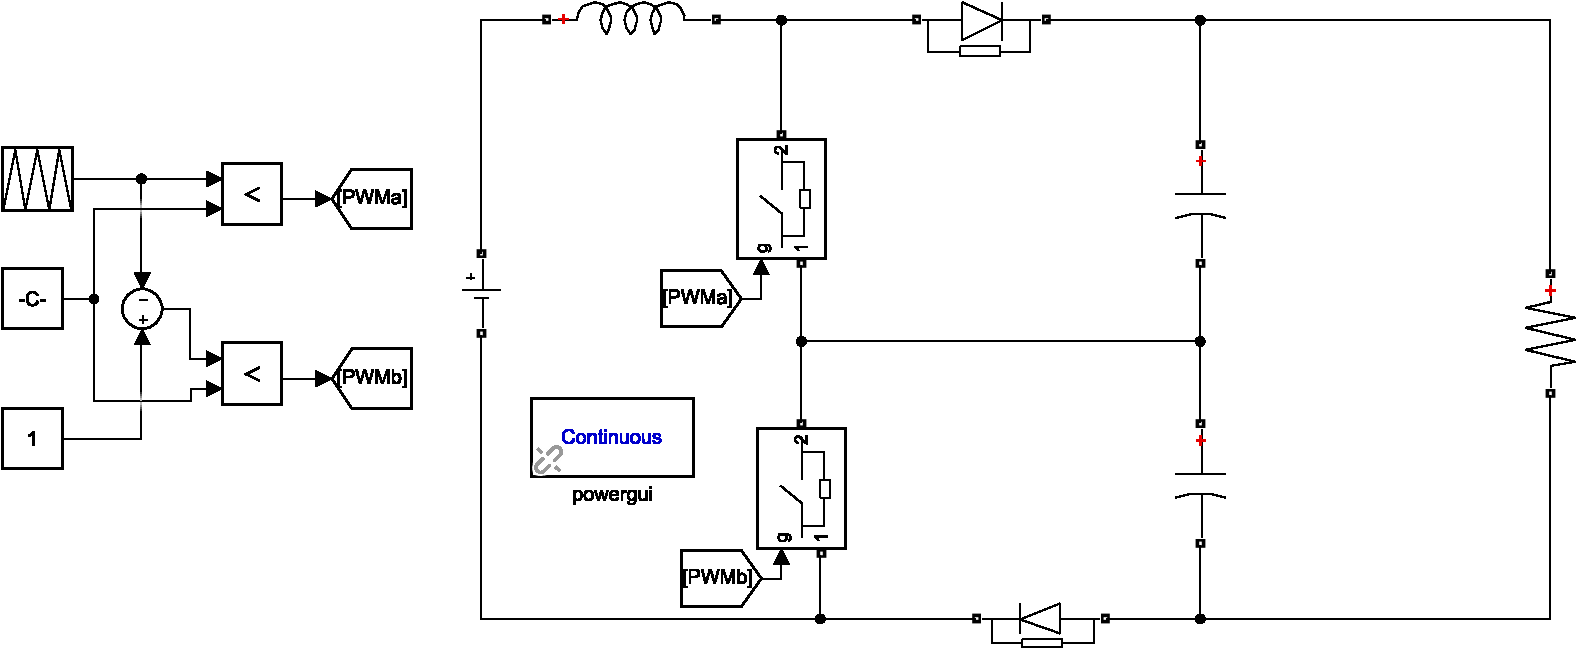
\includegraphics[width=0.8\textwidth]{figures/dConventionalThreeLevelBC/Model_CTLBC.pdf}
    \caption{Switched inductor boost converter SIMULINK Model}
	\label{fig:Model_CTLBC}
\end{figure}

Expected output voltage $V_O$ is calculated using Eq. \ref{eq:CTLBC_CASE2_5} to calculate the gain and multiplying it by $V_{in}$: 
\begin{equation}
	{V_o}= \frac{1}{1-0.6}10=25V
	\label{eq:Simulation_CTLBC}
\end{equation}

The simulation results show the system output is as expected, as observed on Figure. \ref {fig:Simulation_CTLBC}. Voltage levels converge at 25 V. The overshoot and ripple can be compared favourably to a conventional BC with the same parameters. 


\begin{figure} [H]
   \centering
   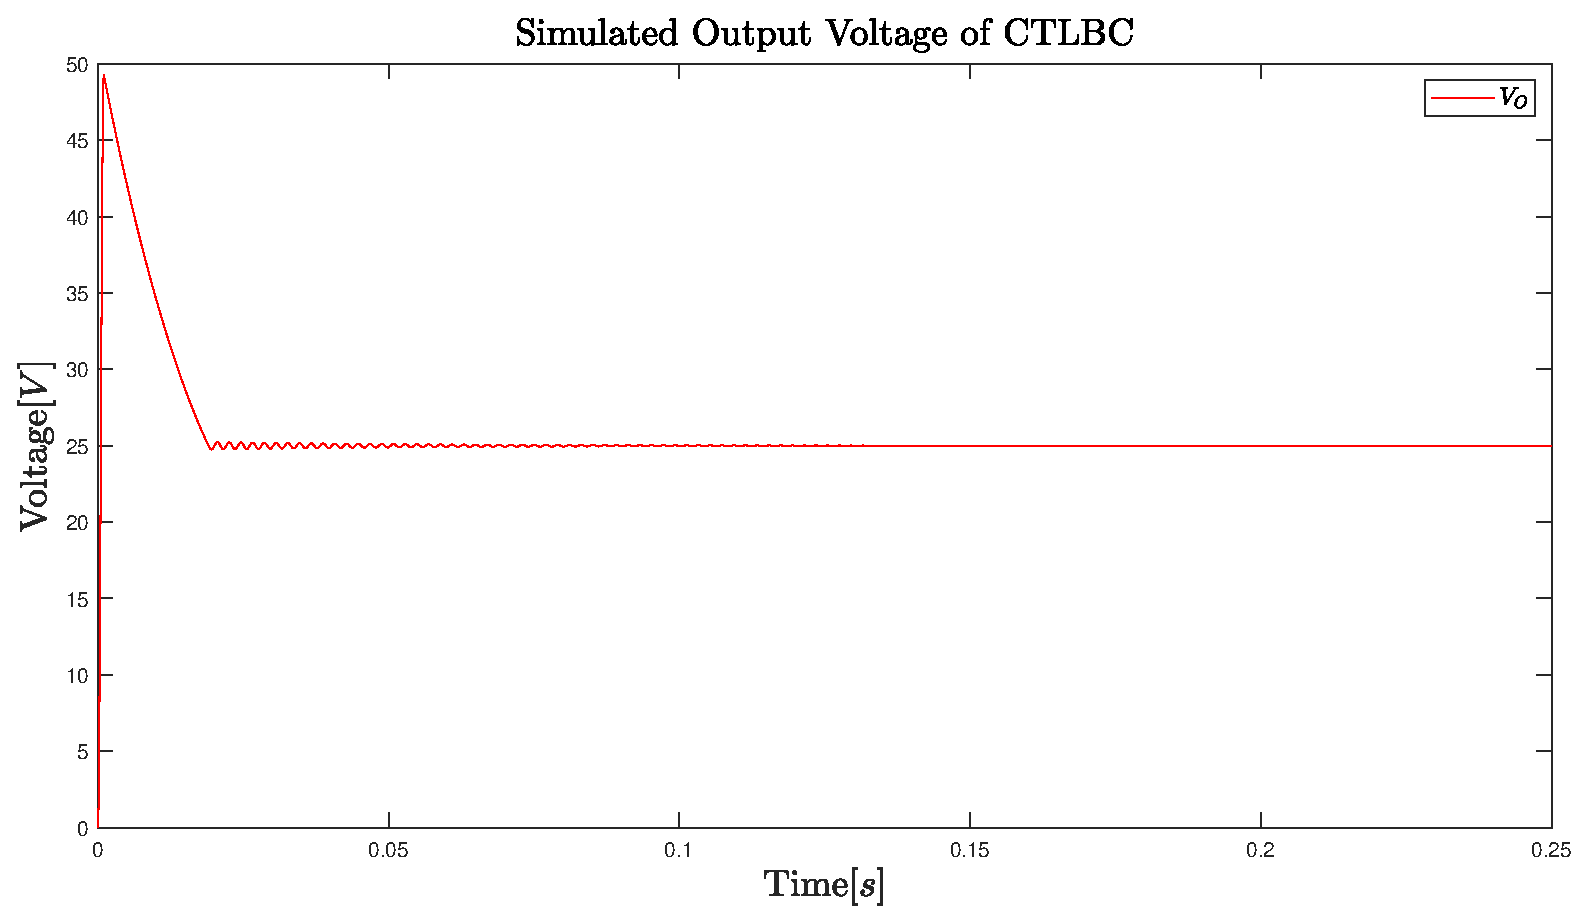
\includegraphics[width=0.8\textwidth]{figures/dConventionalThreeLevelBC/Simulation_CTLBC.eps}
    \caption{Switched inductor boost output voltage}
	\label{fig:Simulation_CTLBC}
\end{figure}